\def\vector#1{\mbox{\boldmath $#1$}}

%!TEX root = ../thesis.tex
%*******************************************************************************
%****************************** Forth Chapter **********************************
%*******************************************************************************
\chapter[演習問題に転用可能なGitHubのイシューの抽出]{演習問題に転用可能なGitHubのイシューの抽出}
\graphicspath{{Chapters_implementation/Figs/}}

\label{section:issue-classification}



\section{実現を目指すシステム}

\begin{figure}[tb]
    \centering
    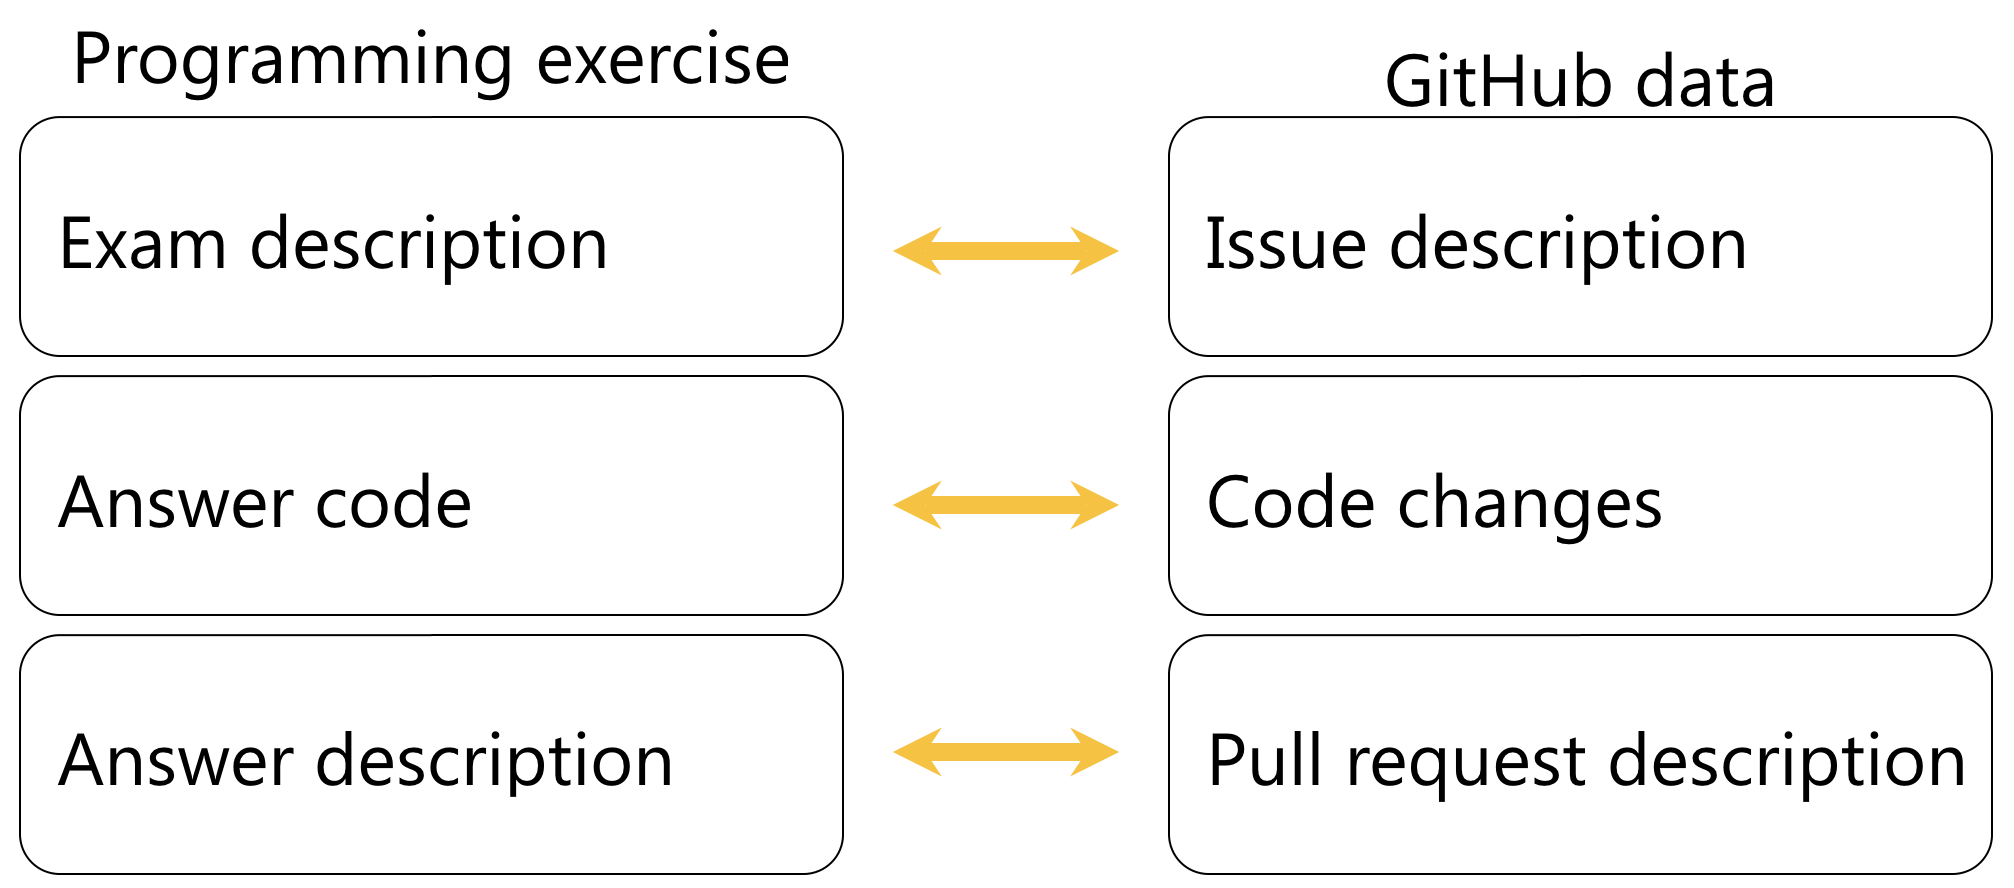
\includegraphics[width=0.9\columnwidth]{system_diagram.png}
    \caption{GitHubのイシューとプルリクエストをプログラミング演習問題へと転用するシステムの概念図.プログラミング演習問題とその解答の説明文を,イシューとプルリクエストの説明文から生成する.さらに解答となるソースコードをプルリクエストのコード変更から生成する.}~\label{fig:system_diagram}
\end{figure}

現実のソフトウェア開発において行われたソースコードの変更データを収集するために,本研究ではソフトウェア開発を管理するウェブ上のプラットフォームであるGitHub~\footnote{\url{https://github.com}}のイシューとプルリクエストを使用する.
GitHubが提供するイシューは,ソフトウェア開発における課題を登録し管理する機能である.
イシューを導入することにより,新機能開発や修正すべきバグといった対応すべき課題を開発チーム内にて円滑に共有することが可能となる.
イシューはタイトル・説明文・ラベルなどの情報から構成される.
GitHubのプルリクエストと呼ばれる機能は,イシューを解決するためのコード変更を管理する機能である.
プルリクエストはタイトルや説明文などのイシューと同様の情報に加えて,イシューを解決するためのコード変更の情報から構成される.

多くのソフトウェア開発者がGitHubを利用しており,2016年9月から1年の間に約1200万件のイシューが作成された~\footnote{\url{https://octoverse.github.com/}}.
従ってGitHubには実践的なソースコード変更の膨大なデータが蓄積されており,それらからプログラミング演習問題を生成し提供することで,より実践的な情報技術の習得を支援することができると考えられる.
本研究が提案するイシューとプルリクエストをプログラミング演習問題へと転用するシステムの概念図を図\ref{fig:system_diagram}に示す.
イシューの説明文は対応すべきソフトウェア開発の課題を説明し,その課題を解決するために必要なコード変更はプルリクエストに含まれている.
プログラミング演習問題も同様に,解答すべき課題の説明と,その解答となるソースコードから構成される.
従って,イシューとプルリクエストからプログラミング演習問題に適した情報を抽出することで,半自動的にプログラミング演習問題を生成することが出来ると考える.


\section{データ収集とヒューリスティクスによる事前処理}

% Our goal is to create programming exercises using issues and code diffs on GitHub, and provide learning experience grounded to real development.
本研究の目的は,GitHubのイシューとプルリクエストを転用することで,実際のプログラミング開発で行われたコード変更を演習問題として提供することにある.
% However, not all the issues and code diffs available on GitHub are appropriate for exercise use.
しかし,GitHub上の全てのイシューやプルリクエストが演習問題への転用に適しているとは限らない.
% For instance, issues may contain lengthy code revisions.
例えば説明のないイシューや,リポジトリに関する専門的な知識を必要とするプルリクエストは,学習者にとって理解することが難しいことが想定される.
% \masaki{例えば説明のないイシューや,リポジトリに関する専門知識を含むプルリクエストは,学習者にとって理解することが難しい.}{「説明のない」がどこまでかかるのか最初分からなかったので,イシューやの後に読点があった方が良いかも?}
% Issues without descriptions would be difficult for a third person to understand their objectives.
% Exercises that require special knowledge about a project or are unnecessarily complex would be inappropriate as well.

% Because of an enormous number of issues and code diffs on GitHub, we performed screening before performing classification.
そこで我々は,GitHub上の公開されているイシューとプルリクエストのうち,プログラミング演習問題に転用できると考えられるものを抽出するため,以下の5つのヒューリスティクスを用いた.
\begin{enumerate}
\item[H1] \textbf{リポジトリ外部の開発者でも対応可能と明示的に指定されているイシューであること}: この情報がイシューに対して明示的に与えられていることは,コード変更に必要な情報が全てイシュー内で提供されていると想定できるため.
\item[H2] \textbf{プルリクエストに含まれるコード変更が50行以下であること}: 極端に長いコード変更は演習問題として不適切であるため.
\item[H3] \textbf{プルリクエストのコード変更が1ファイルのみにて行われていること}: 複数のファイルにまたがるコード変更は各ファイルの役割などリポジトリ特有の知識を必要とする可能性が高いため.
\item[H4] \textbf{イシューが説明文を含むこと}: 説明文をプログラミング演習問題の問題文として利用するため,その情報がないイシューは不適切であるため.
\item[H5]  \textbf{イシューが閉じられており,関連するプルリクエストがマージされていること}: マージはコード変更が開発チームで認めれたものであり,コード変更が適切であることを示すと考えられるため.
\end{enumerate}

\begin{figure}[t]
    \begin{tabular}{c}
      %-------------------------------
      \begin{minipage}[t]{0.5\columnwidth}
        \centering
        
        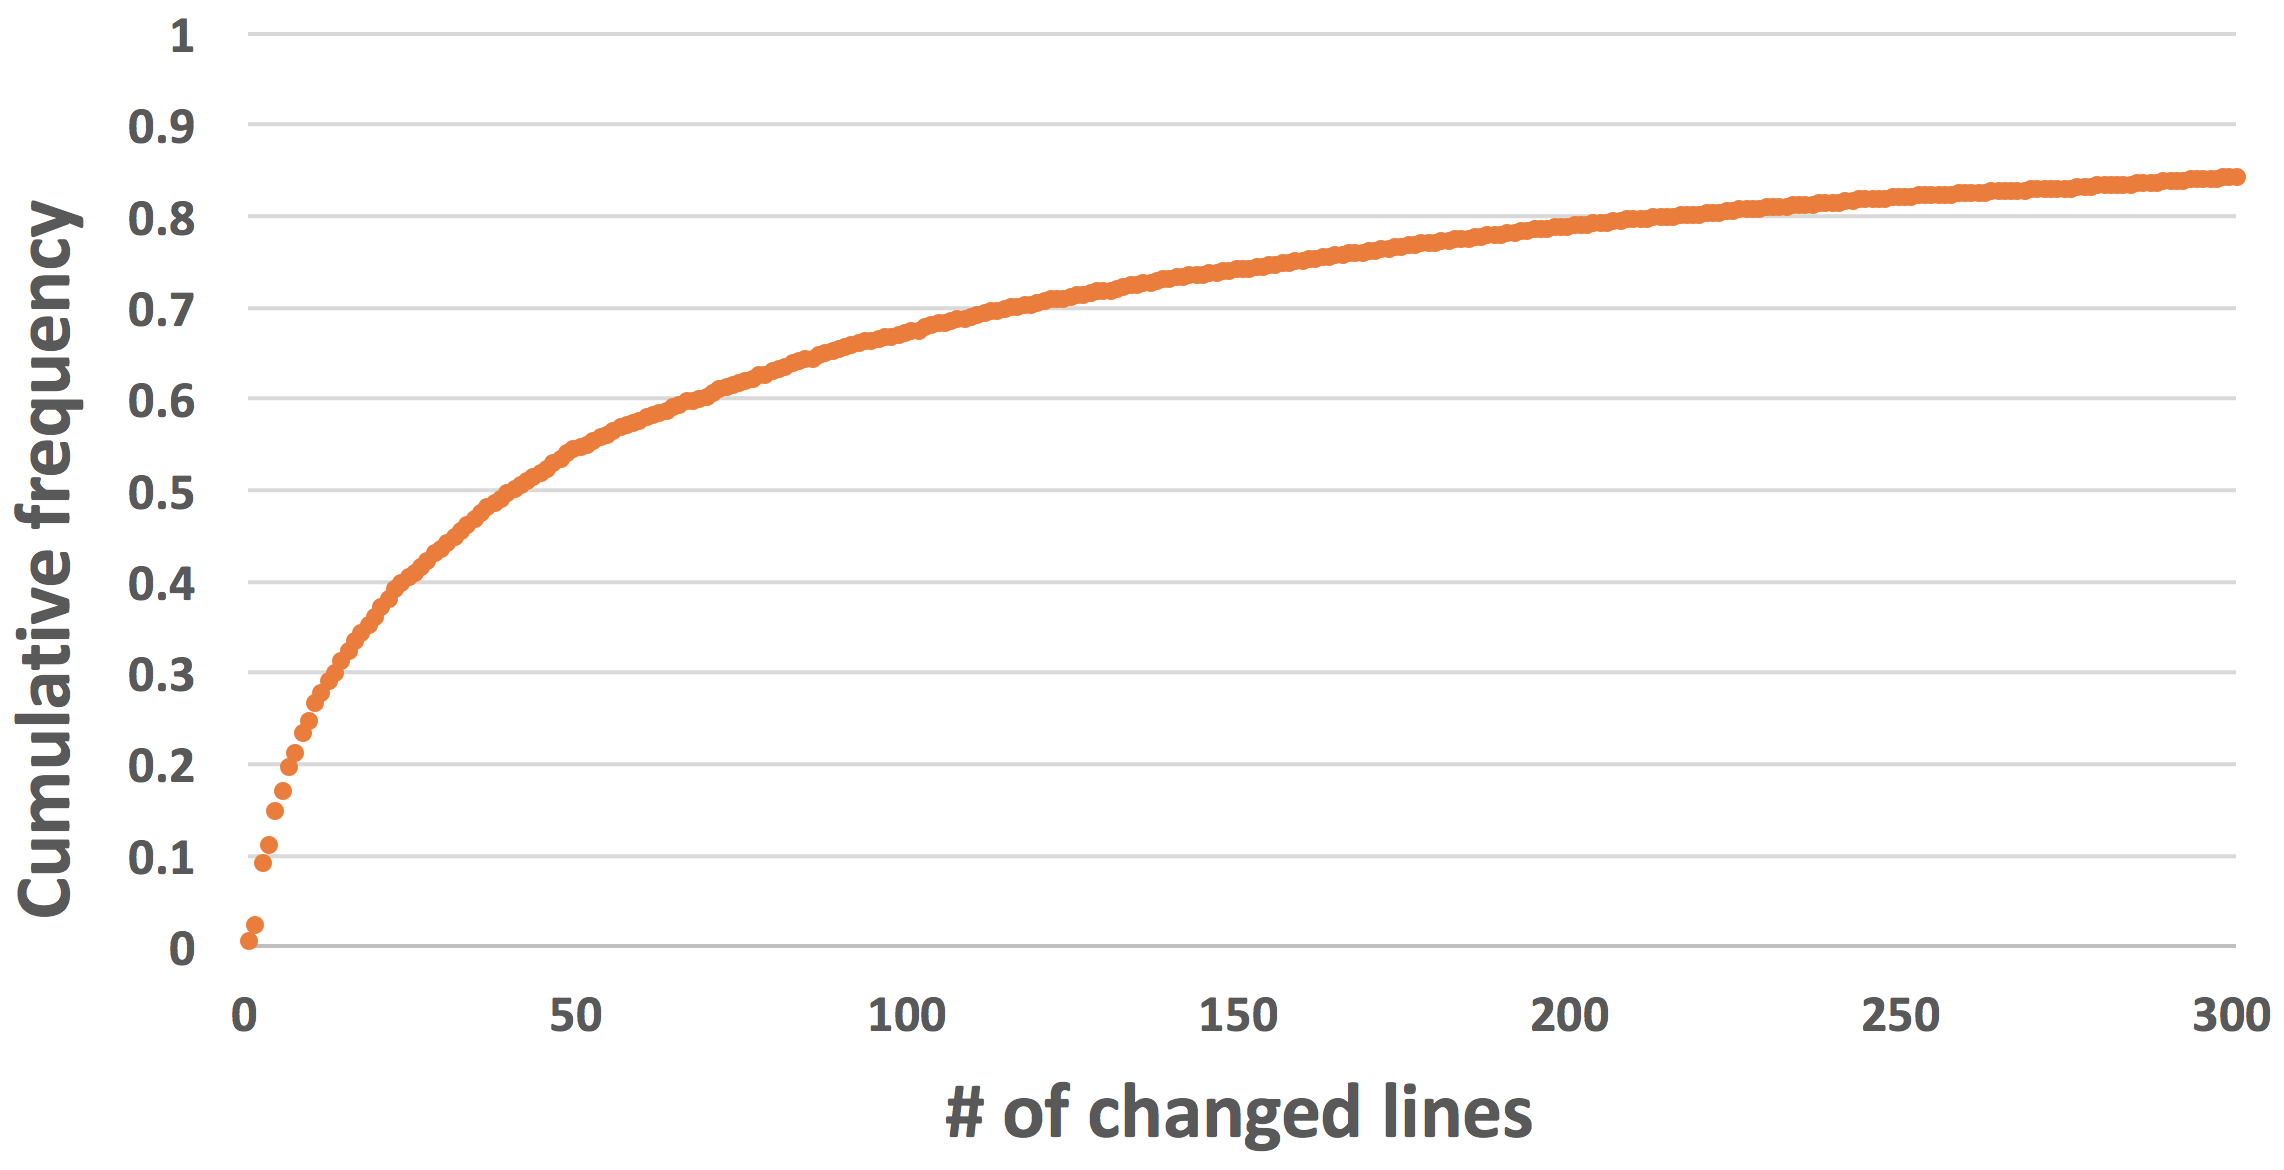
\includegraphics[width=0.95\columnwidth]{histogram_changes.png}
        \subcaption{コードの変更行数の累積分布.}~\label{fig:histogram_changes}
      \end{minipage}
      
      \hspace{0.05cm}
      
      %------------------------------
      \begin{minipage}[t]{0.5\columnwidth}
        \centering
        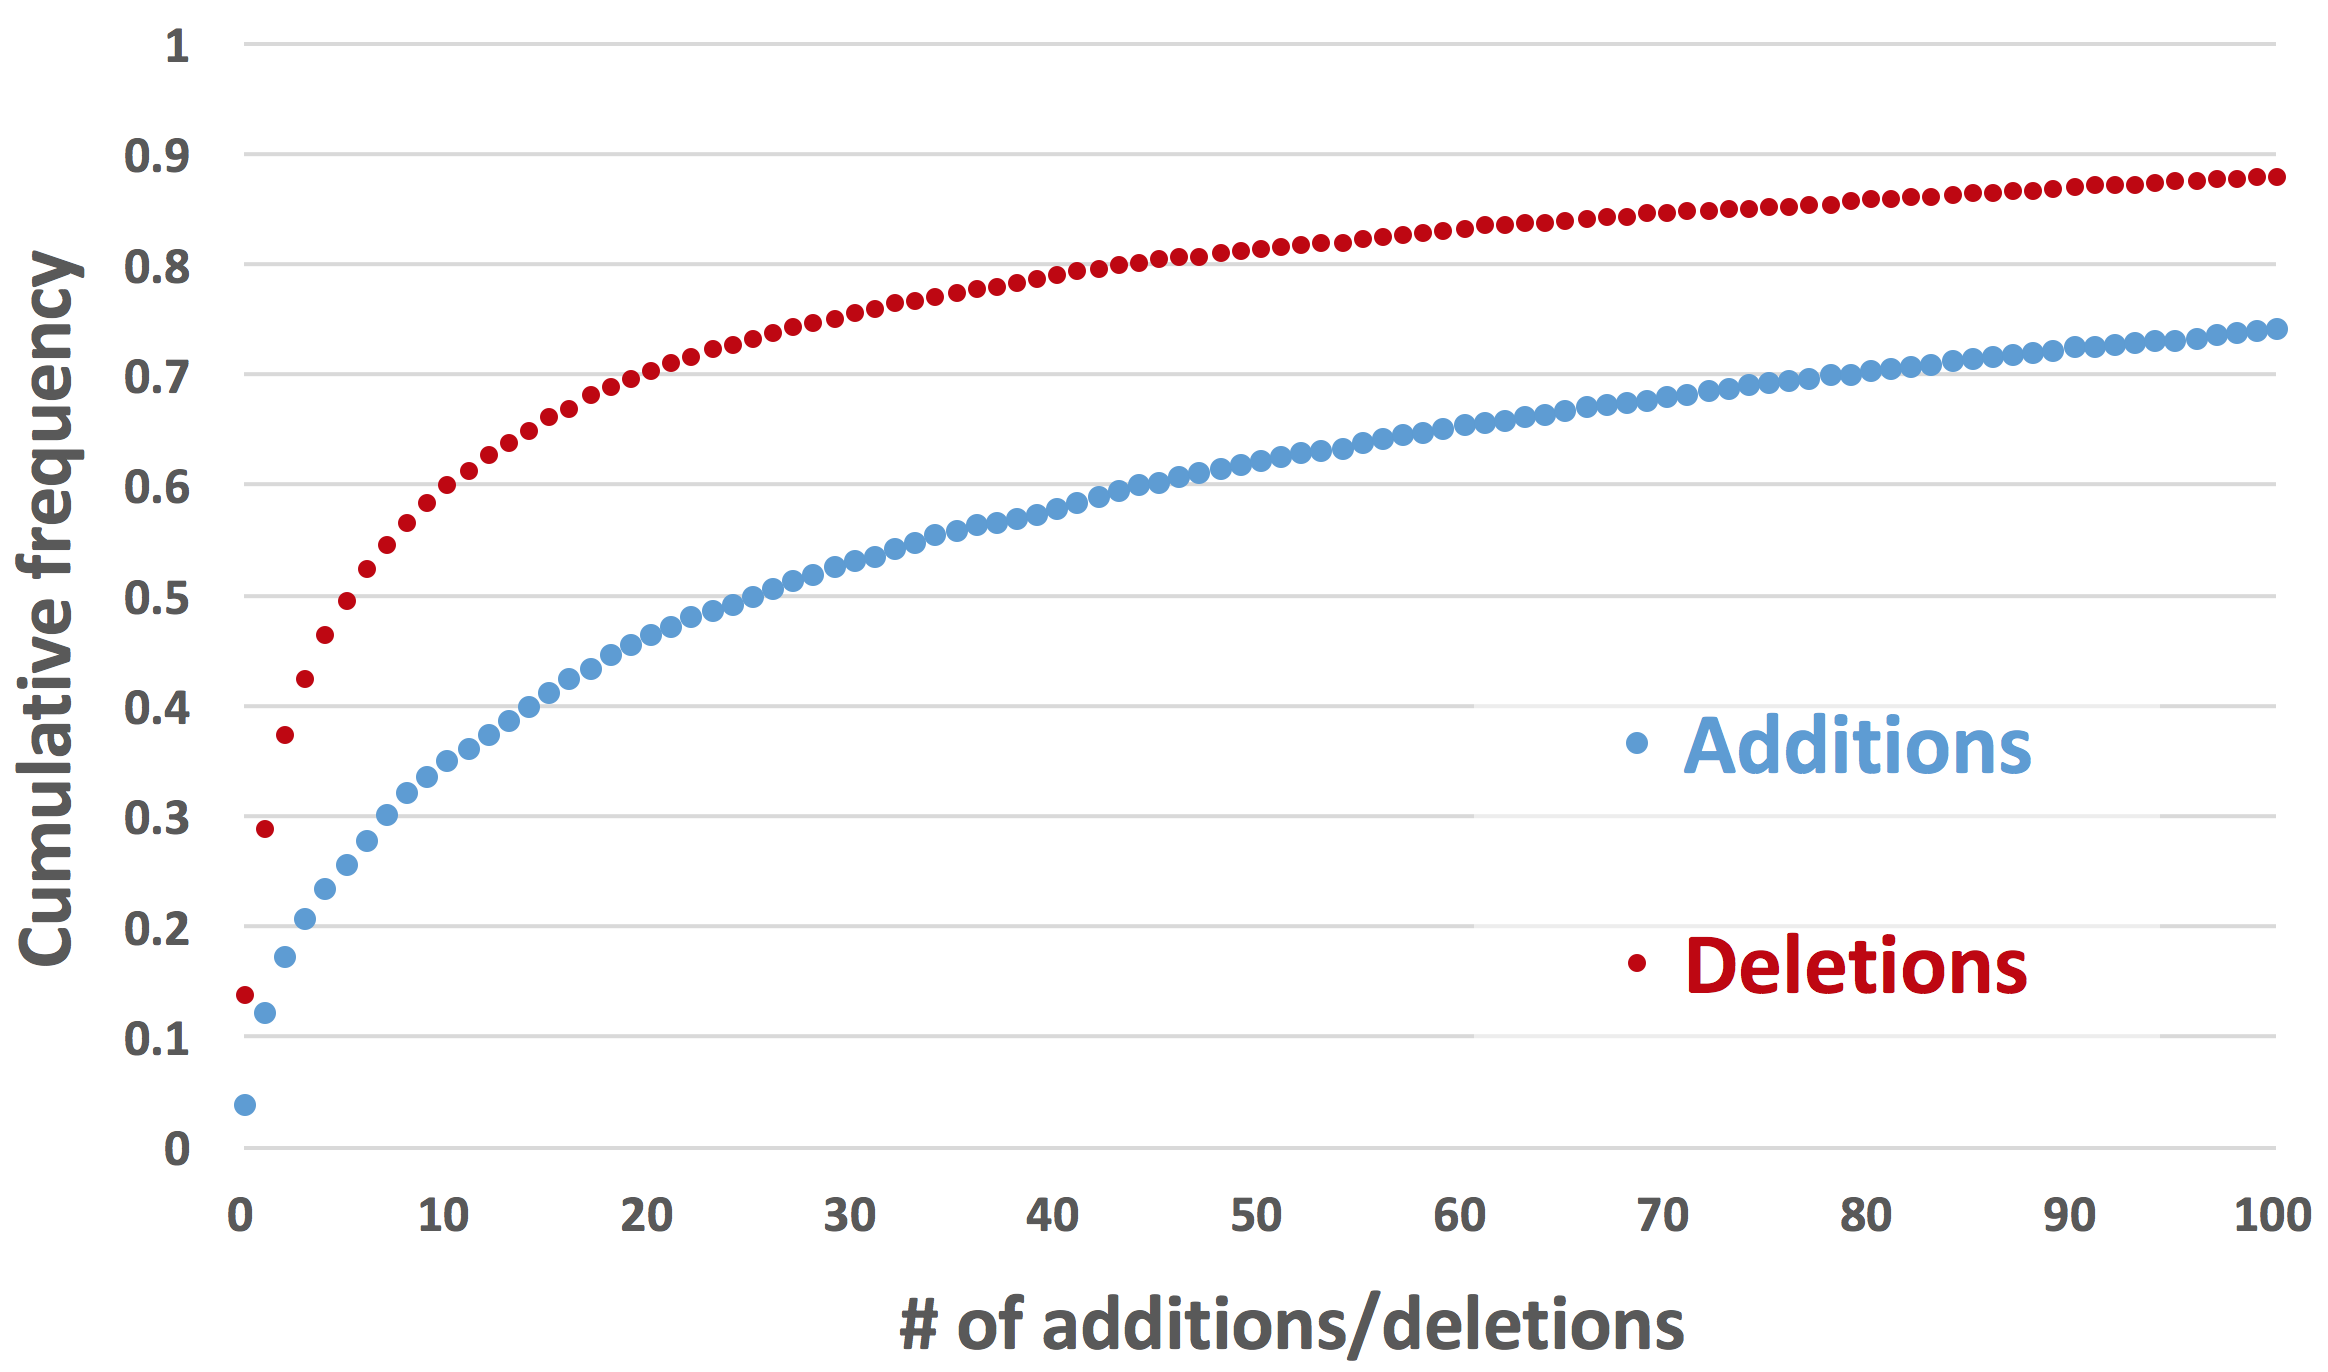
\includegraphics[width=0.92\columnwidth]{histogram_adds_dels.png}
        \subcaption{コードの追加および削除行数の累積分布.}~\label{fig:histogram_adds_dels}
      \end{minipage}
      
      \\
      
      %------------------------------
      \begin{minipage}[t]{0.5\columnwidth}
        \centering
        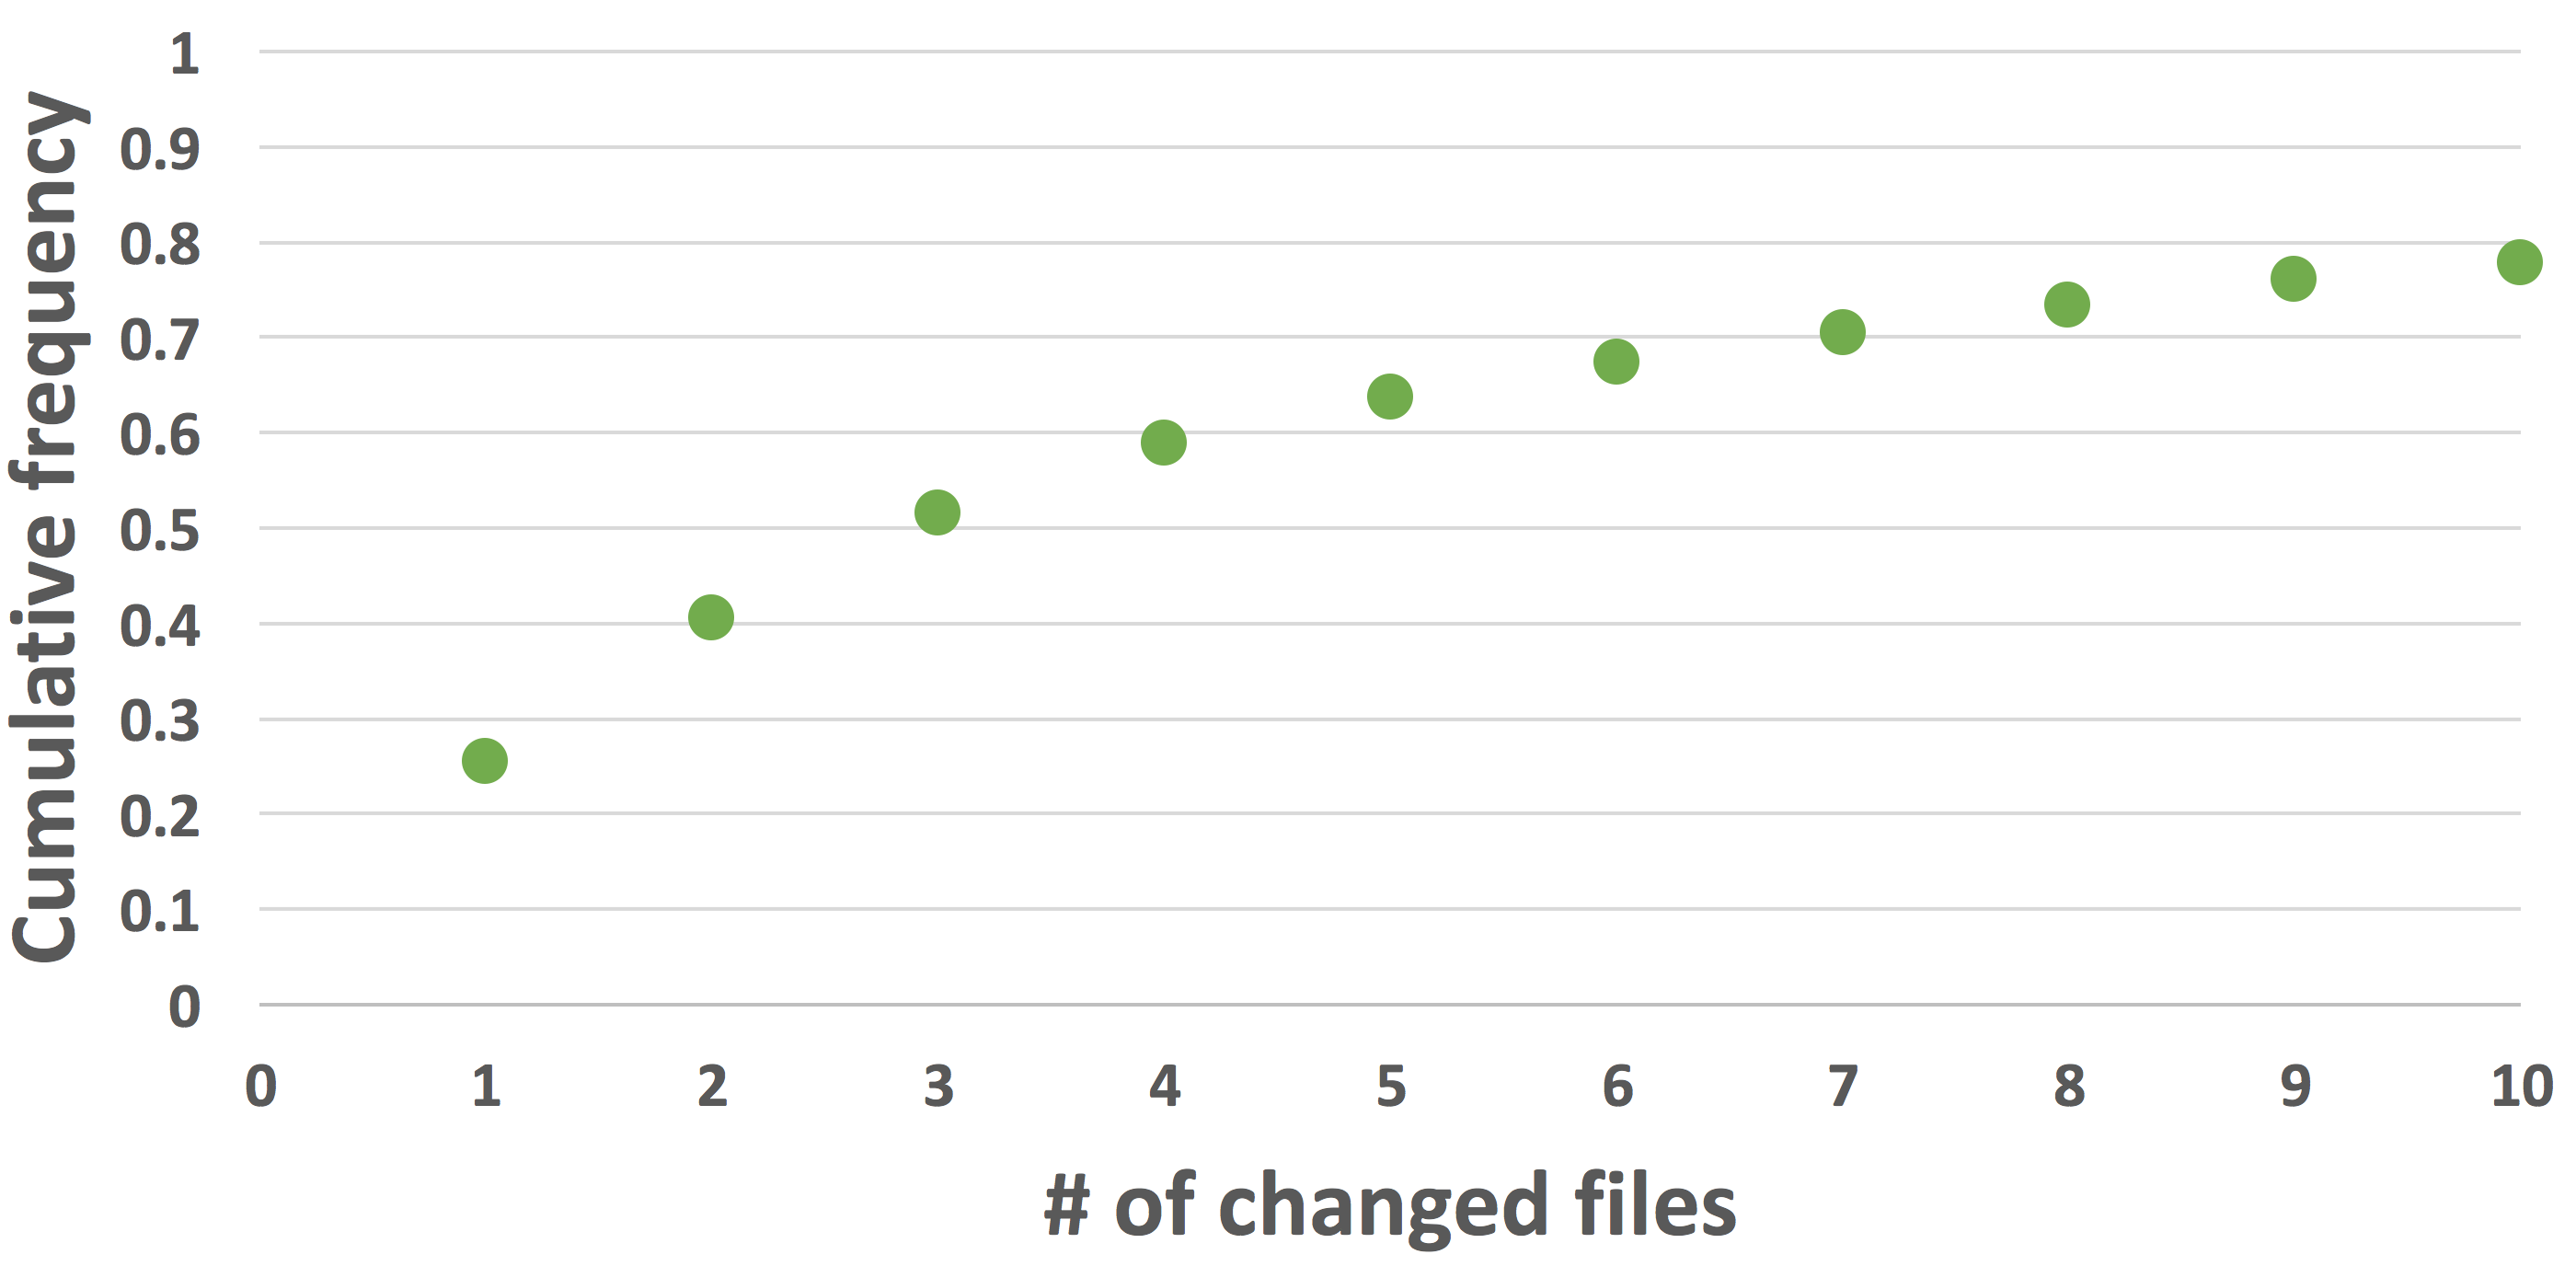
\includegraphics[width=1.0\columnwidth]{histogram_changed_files.png}
        \subcaption{変更ファイル数の累積分布.}~\label{fig:histogram_changed_files}
      \end{minipage}
     
    \end{tabular}
    \caption{プルリクエストによって変更されたコード変更の行数,追加および削除行数,および変更ファイル数の累積分布.}
\end{figure}

Up for grabs\footnote{\url{http://up-for-grabs.net}}というウェブサイトでは,リポジトリ外部の開発者であっても取り組むことができるイシューを列挙している.
我々はこのウェブサイトが掲載しているラベル(例えば``good first issue''や``help-wanted'')が付けられているイシューのみを利用することで,H1を適応することとした.
また,データ収集時にクエリを使用することで,H4とH5に対応した.
その結果,2018年3月12日の時点で更新が新しい順に3,000件のリポジトリから,H1,H4,H5を満たすイシューと関連するプルリクエストを取得した.
% 成果輪講の話
次に,H2とH3を満たすイシューがどの程度存在するのかを検証するために,収集したプルリクエストにて行われたコードの変更行数の分析を行った.
プルリクエスト内にて変更された行数の累積分布を図\ref{fig:histogram_changes}に,追加・削除された行数の累積分布を図\ref{fig:histogram_adds_dels}に,変更されたファイル数の分布を図\ref{fig:histogram_changed_files}に示す.
以上の分析により,GitHubから収集したイシューと関連するプルリクエストのうち6,381件(1.6\%)がH2とH3を満たすことが明らかとなった.
それらのイシューを抽出することでデータセットを構築した.
% そしてそれらのイシューにH4とH5を適用した結果,6,381件のイシューと関連するプルリクエストを抽出した.

% Data collecting
%%%%%%%%%%%%%%%%%%%


\begin{figure}[tb]
    \centering
    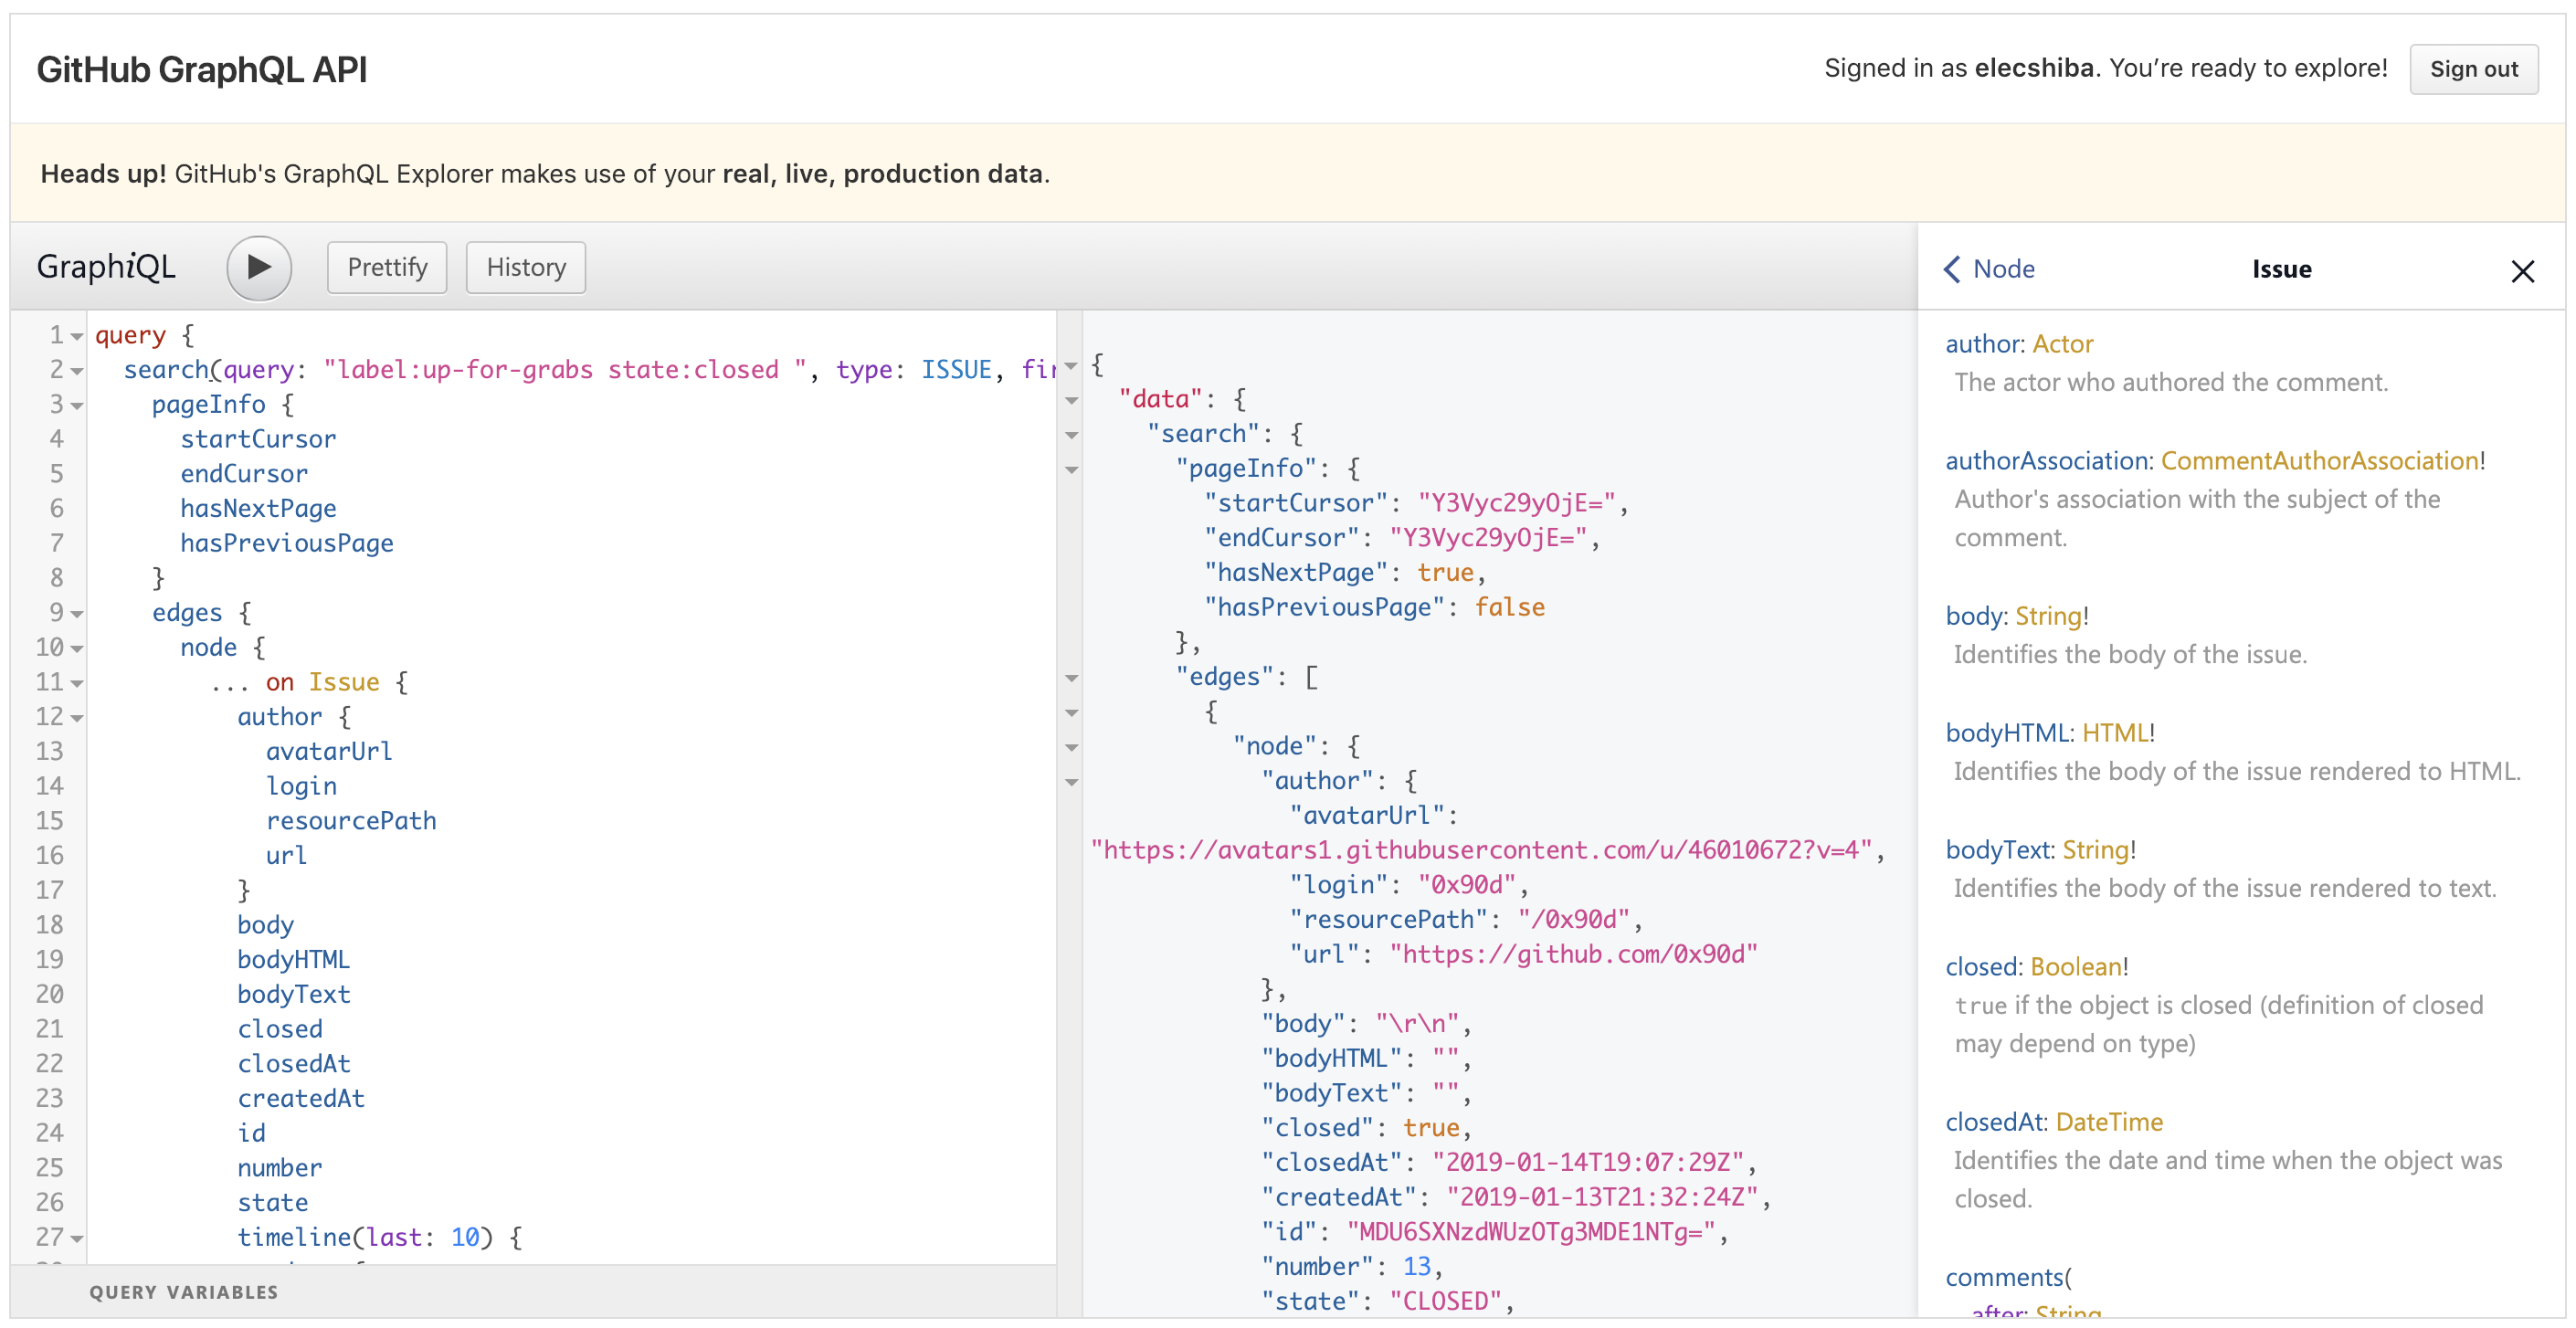
\includegraphics[width=1.0\columnwidth]{GitHub_api_explorer.png}
    \caption{GitHub GraphQL API Explorer~\footnote{\url{https://developer.github.com/v4/explorer/}}にて,データ収集用のクエリを実装している様子.左のエディタ上で実装したクエリを実行した結果が中央に表示されている.また,使用可能なスキーマやフィールドのドキュメントを右側のパネルで閲覧できる.}~\label{fig:GitHub_api_explorer}
\end{figure}


\begin{table}[t]

  \centering
  \caption{GitHubから収集したデータの構造}
  \label{table:format_collected_GH_data}
    
  \begin{tabular}{l | c | c } \Xhline{3\arrayrulewidth}
      名前 & 型 & 説明 \\ \hline \hline
      author & json & ユーザ名やユーザページのURLなど\\
      body & string & イシューの説明文  \\
      bodyHTML & string & HTML表記でのイシューの説明文 \\
      comments & [json] & コメントの本文や作成者の情報など \\
      createdAt & datetime & イシューが作成された日時 \\
      labels & [json] & イシューに付与されているラベルに関する情報 \\
      repository & json & リポジトリ名やURL,主要な開発言語など\\  
      state & string & イシューの状態(open,closedなど) \\
      pullRequest & json & プルリクエストの説明文やコード変更量など \\
      title & string & イシューのタイトル \\
      url & string & イシューのURL \\
      
      \Xhline{3\arrayrulewidth}
  \end{tabular}
\end{table}

GitHubからのデータ収集にはGitHub GraphQL~\footnote{\url{https://developer.github.com/v4/}}を使用した.
GraphQLではデータの構造とフィールドを指定することで,必要な情報のみを取得することができる.
また,イシューに関連するプルリクエストといった,関連する異なるオブジェクトをも1クエリで取得することができるという特徴をもつ.
図\ref{fig:GitHub_api_explorer}にGitHub GraphQL API Explorer~\footnote{\url{https://developer.github.com/v4/explorer/}}にてクエリを実装している様子を,表\ref{table:format_collected_GH_data}にデータ収集にて使用したデータ構造を示す.
型がjsonの項目については,その項目に関する必要な情報がネスト形式で記述されている.

\begin{figure}[t]
  \centering
  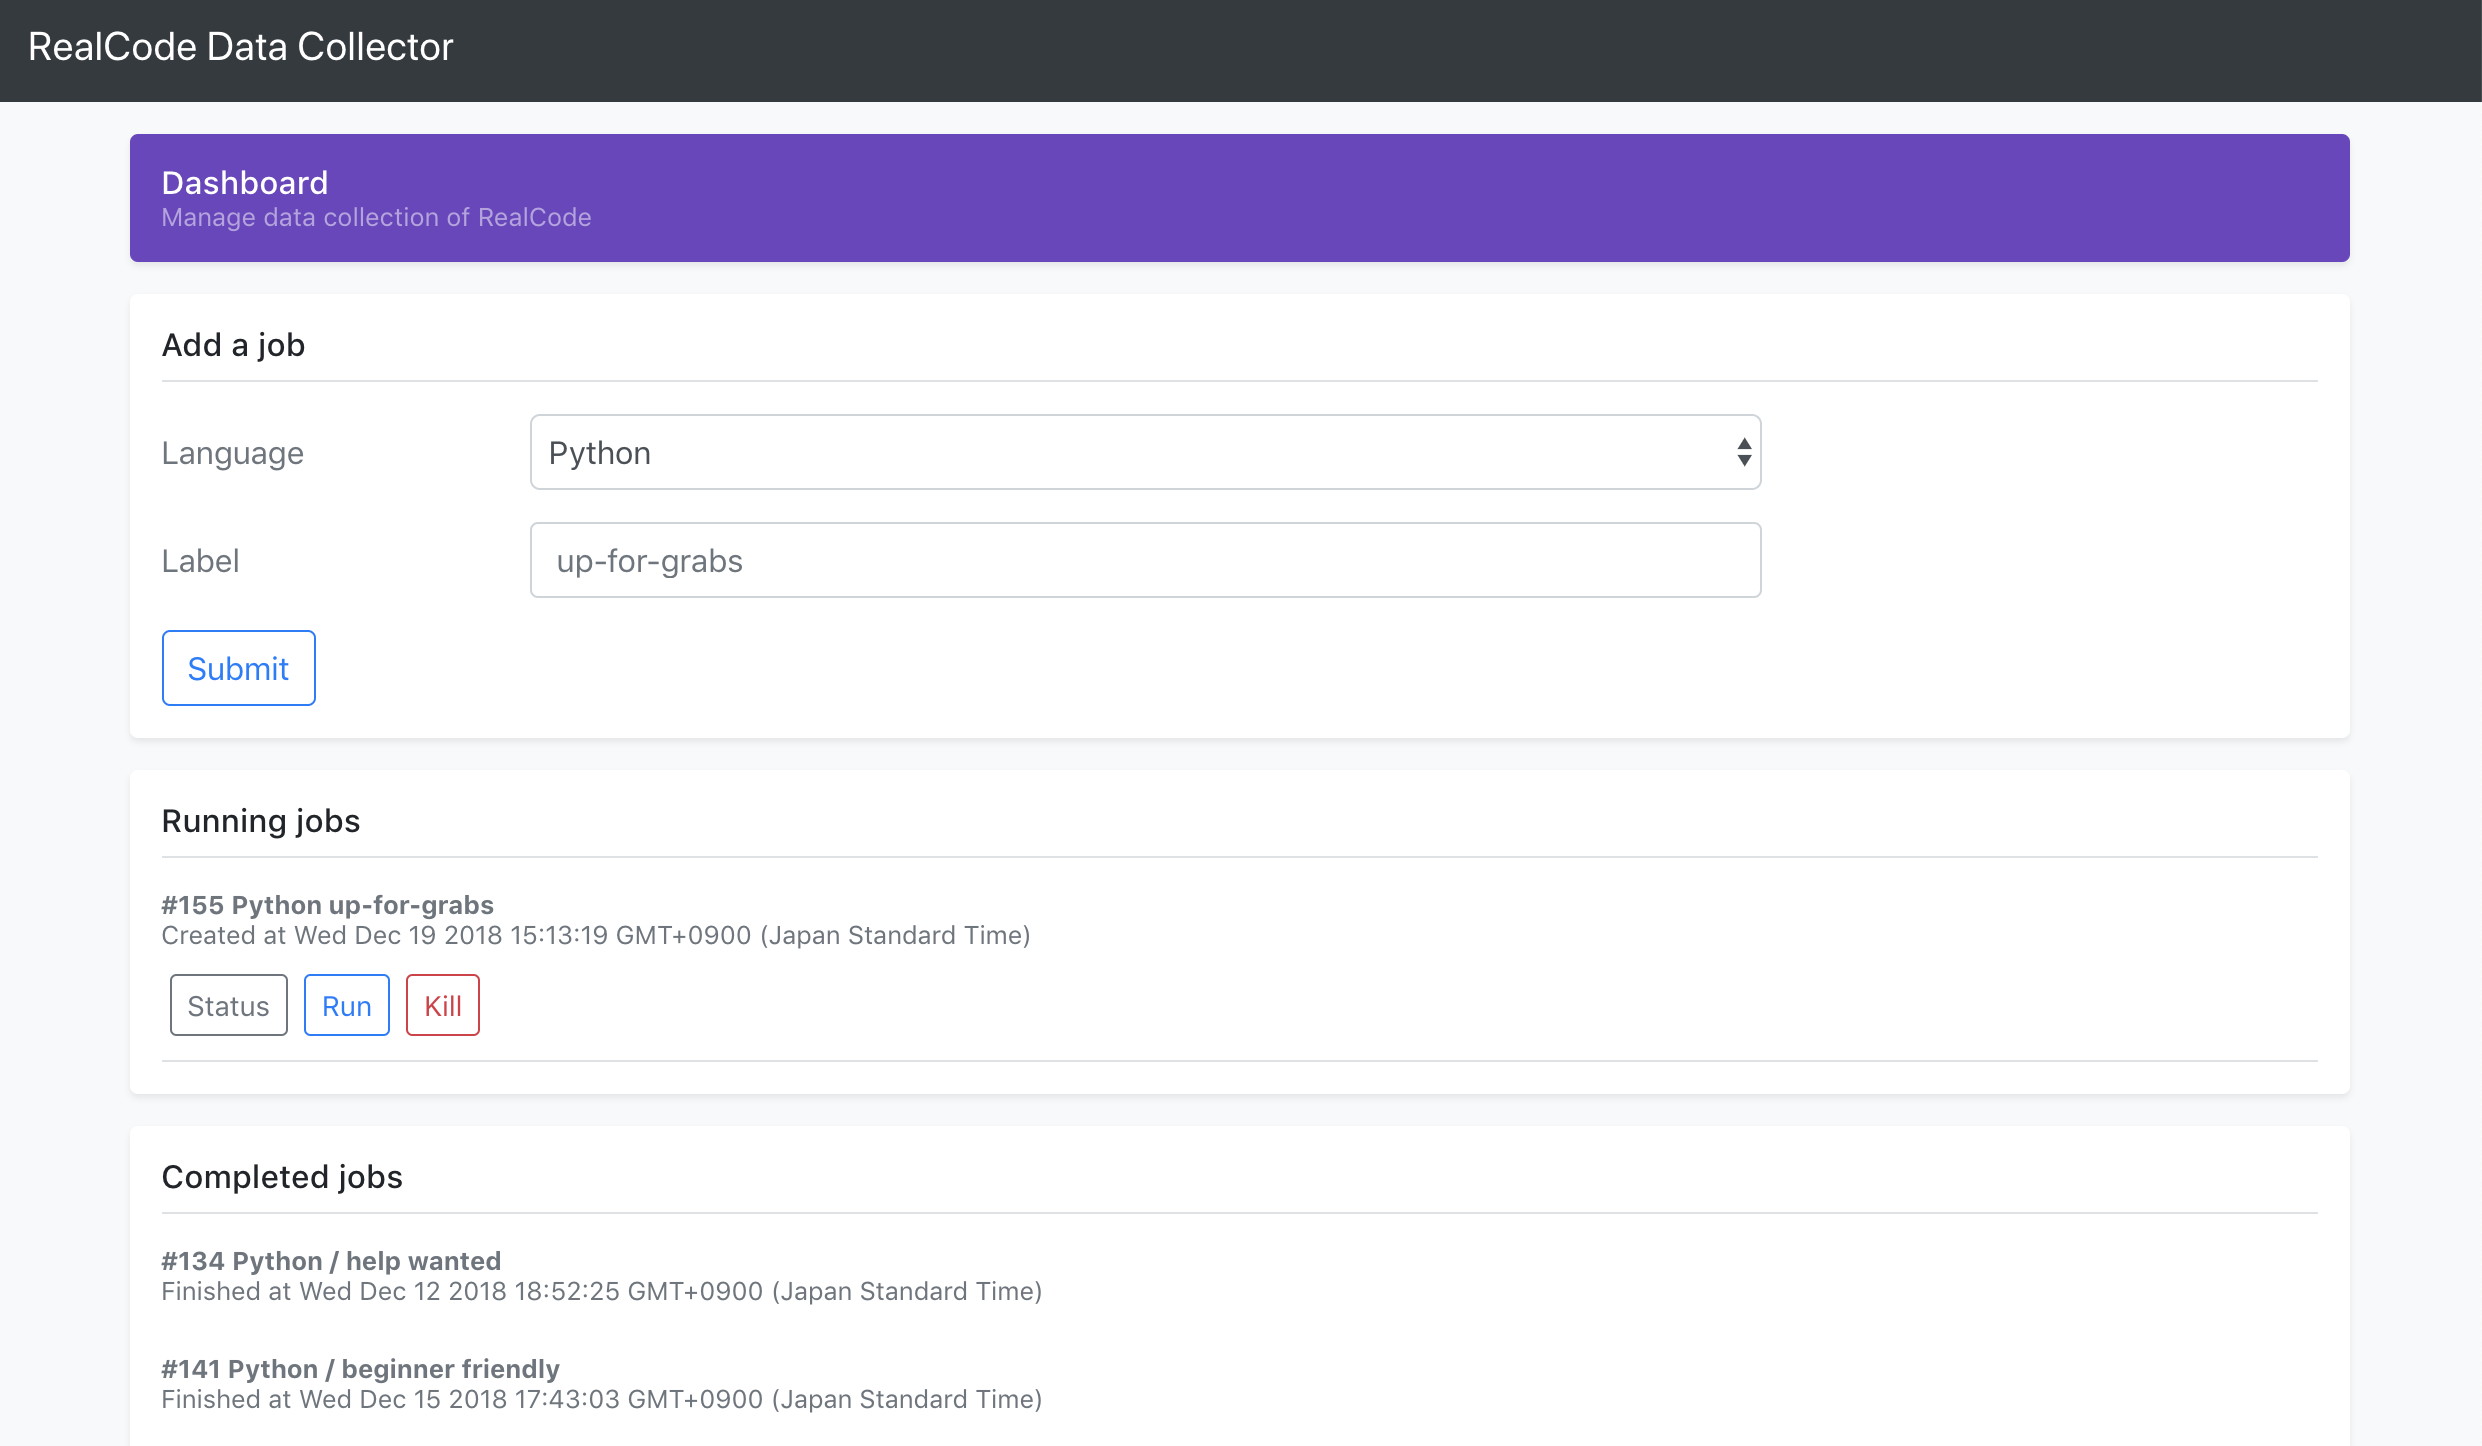
\includegraphics[width=1.0\columnwidth]{realcode-data-collector-screenshot.png}
  \caption{RealCode用のデータ収集管理画面.}
  \label{fig:realcode-data-collector}
\end{figure}

図\ref{fig:realcode-data-collector}に,GitHubからのデータ収集を管理するために開発したシステムのインターフェースを示す.
``Add a job''というタイトルのフォームにて収集するデータのプログラミング言語とイシューのラベルを指定することで,バックグラウンドにてデータ収集のジョブを実行する.
バックグラウンドでジョブを実行するためにKue\footnote{\url{https://github.com/Automattic/kue}}というライブラリを,ジョブの状態を管理するためにRedis\footnote{\url{https://redis.io/}}というインメモリDBを使用している.
実行中のジョブは図\ref{fig:realcode-data-collector}の``Running jobs''に,完了したジョブは``Completed jobs''にそれぞれ表示されている.

GraphQLによりイシューと関連するプルリクエストの情報を抽出することができるが,プルリクエストにて行われた実際のコード変更データはGraphQLからは取得することができない.
GraphQLから収集したイシューについて,gitコマンドを用いて関連するリポジトリとコード変更履歴をクローンし,変更前と変更後のバージョンのコードを比較することでコード変更データを抽出した.
Pythonからgitコマンドを実行するために,GitPython~\footnote{\url{https://gitpython.readthedocs.io/en/stable/}}を使用した.

  
\section{決定木を用いた転用に適したイシューの抽出}

\subsection{データのラベル付け}
前節にて述べたGitHub上のデータ抽出作業により,プログラミング演習問題に転用する上で不適切であると考えれるイシューおよびプルリクエストを取り除くことができた.
しかし,抽出されたデータから作られた演習問題がすべて適切であるとは限らない.
例えばソースコード中のコメントを修正するような演習問題は,プログラミング言語の学習において学べることは非常に小さい.
そこで我々は妥当でないプログラミング演習問題を生成し得るイシューを除去するための,機械学習を用いた分類器を実装することとした.
%また,分類器の学習に必要なデータセットを構築するために,学生によるラベル付けを行った.

% Although our screening filtered out issues clearly unusable for our purpose, it is still unknown whether generated exercises would offer valid problems.
% We thus decided to create a classifier to remove issues and code diffs that would result in invalid exercises.
% To this end, we conducted an experiment to collect human ratings.

分類器の実装にあたり,イシューから転用した演習問題がプログラミング演習問題として成立するかどうかの評価を行い,教師あり学習におけるラベルを生成することとした.
まず,事前処理後のデータに修正を加えずに,イシュー内の説明文とコード変更をそれぞれ問題文,解答コード例とするプログラミング演習問題を生成した.
それぞれの演習問題に対し,「与えられた演習問題は,問題として成立していた.」かを,Pythonの授業を大学で受講した経験がある10人の学生(PA1--10)に5段階で評価してもらった(1: 全く同意しない -- 5: 強く同意する).
各実験参加者は時間の許す限りできるだけ多くの演習問題の評価を行ってもらうように指示した.
評価の結果,少なくとも2人の実験参加者が評価を行ったイシューが211件得られた.

% We recruited 10 students (PA1--10) who had taken at least one Python class at their universities.
% During the experiment spanning for three days, we asked the participants to solve at least 50 exercises generated by our system.
% For each exercise, the participants were asked to response to a 5-Likert scale question of ``This was a valid programming exercise.'' (1=Strongly disagree -- 5=Strongly agree).
% %We offered approximately 45 USD in local currency as a compensation at the end of the experiment.
% The participants were also encouraged to solve as many exercises as possible with an incentive of additional compensation for the top three contributors.
% As a result, we collected 211 exercises that contain ratings from 2 participants.

211件のイシューに対して,得られた回答の平均値が3.5点以上のイシューをプログラミング演習問題への転用に適するもの,それ以外を転用に適さないものとした.
その結果,85件の転用に適するイシュー(``repurposeable")と,126件の転用に適さないイシュー(``unrepurposeable")を得た.

% We took the average value for the two ratings on each exercise.
% We then categorized each exercise to ``valid'' if the average was equal to or higher than 3.5.
% The rest of the exercises were grouped to ``invalid" to make our classification rather conservative.
% After categorization, we had 85 and 126 exercises for the valid and invalid categories, respectively.

\subsection{分類手法}
% 
ラベル付けされたプログラミング演習問題の件数が限られているため,本研究では決定木を用いた分類器を利用することとした.
決定木は分類の工程や結果を可視化することができるため,どの特徴量が分類に有効であるかどうかを議論することが可能となる~\cite{FRIEDL1997399}.

% Data-intensive methods (e.g., deep learning) would be infeasible due to the small size of our dataset. 
% We instead decided to use a decision tree (a Classification and Regression Tree) for our classification.
% A decision tree also visualizes classification process, and we can examine what features would contribute to accurate classification.

はじめに我々はunrepurposeableと分類されるべきイシューを特定するための次の3つの仮説を立てた.
% \sakaguchi{}{これは上の実験のインタビュー結果からでしょうか?}
\begin{itemize}
\item[\textbf{仮説1}: ] \textbf{コード変更が短すぎる.} コードの変更量が少なすぎるものは含まれている学習すべき内容が少ないと想定されるため.
\item[\textbf{仮説2}: ] \textbf{イシューの説明文が短すぎる,あるいは長すぎる.} 説明文が短いものは問題内容を理解するためには十分な情報が入っていない,長過ぎるものは問題内容を読むこと自体に時間がかかりすぎてしまうと想定されるため.
\item[\textbf{仮説3}: ] \textbf{イシューを取得してきたリポジトリが,リポジトリ外部の開発者向けのイシューを頻繁には作成していない.} このようなリポジトリでは,リポジトリ外部の開発者との連携が少なく,外部の開発者向けのイシューの難易度,説明文の情報量に関する十分な経験がないと考えられるため.
\end{itemize}

% To derive potential features, we first derived the following hypotheses for identifying issues to be removed: H1) A code diff causes syntax errors; H2) A code diff is too short; H3) A description is too long or too short; and H4) The associated repository rarely creates entry tasks for external contributors.

上記の仮説を元に,我々は次の3つの特徴量を作成した.

% The second hypothesis is derived because too short code diff would not hold much information to learn.
% We expect that descriptions in a repository which rarely creates issues for external basic-level contributors may not be easy for non-members to understand.
% Based on these hypotheses, we created the four following features:

\begin{itemize}
% \setlength{\leftskip}{-3mm}
  \item \textit{code\_lines}: コード変更の行数
  \item \textit{desc\_words}: イシューの説明文の単語数
  \item \textit{entry\_issues}: 各リポジトリにおいて外部の開発者向けと指定されているイシューの数
\end{itemize}

% \begin{itemize}
% \setlength{\leftskip}{-3mm}
%   \item \textit{syntax\_error}: 1 if the portion affected by a code diff causes syntax errors, and otherwise 0.
%   \item \textit{code\_lines}: the number of lines in code diffs.
%   \item \textit{desc\_words}: the number of words in issue descriptions.
%   \item \textit{entry\_issues}: the number of entry issues in the same repository. For this feature, we counted issues listed in Up for Grabs for each repository.
% \end{itemize}

%We calculated the value of these features for all labeled issue and code diff data.

決定木の学習においては,過学習を防ぐために決定木の深さを3以下にし,分類されたサンプルが3つ以下の枝については枝刈りを行った.
決定木の精度の評価には10分割交差検証法を採用した.

% We then trained a decision tree with constraining its depth to be three to avoid over-fitting.
% We also pruned trees that applied to fewer than three samples.
% We conducted 10-fold cross validation for performance measurement.



\begin{figure}[t]
	\centering
  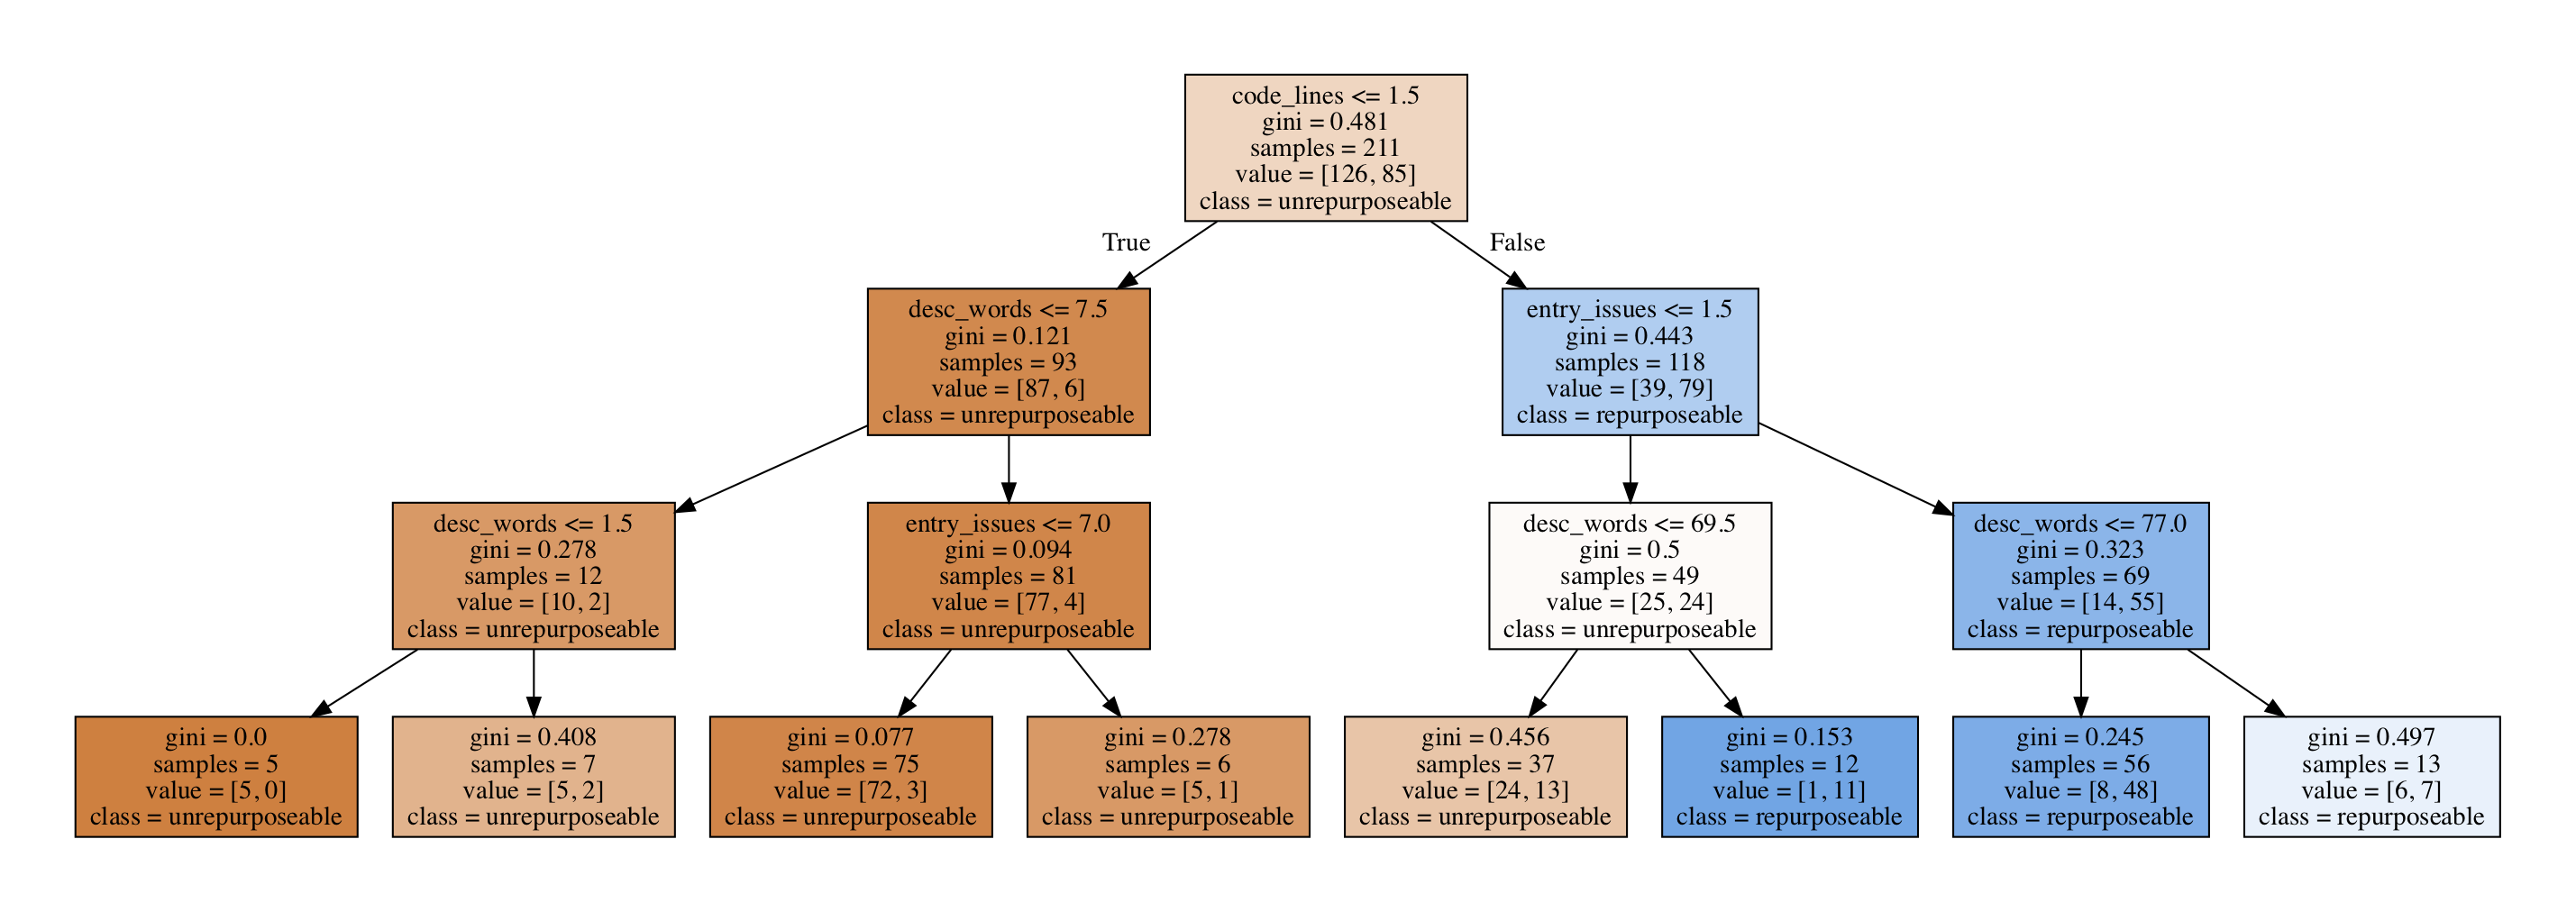
\includegraphics[width=1.0\columnwidth]{graph_20181005.png}
  \caption{プログラミング演習問題への転用に適するイシュー(``repurposeable")と,転用に適さないイシュー(``unrepurposeable")を分類する決定木.背景色が青の葉はrepurposeableへと,橙の葉はunrepurposeableへと分類する.葉の背景色が濃いほど,ジニ係数が小さいことを意味する.}
  \label{fig:dtgraph}
\end{figure}


図~\ref{fig:dtgraph}に211件のラベルづけされた全てのイシューを用いて学習させた決定木を示す.
橙はunrepurposeable,青はrepurposeableとして分類されることを意味する.
10分割交差検証法で識別精度を検証した結果,unrepurposeableな演習問題において適合率が0.89,再現度が0.73,repurposeableなイシューにおいて適合率が0.71,再現度が0.83であった.
図~\ref{fig:dtgraph}が示すように,コード変更の行数を用いた分類が第1段階で行われており,イシューの識別において大きな役割を担っていることが示唆される.
特に,1行のコード変更からなる演習問題の多くがunrepurposeableな演習問題として分類されている.
また,\textit{desc\_words}と\textit{entry\_issues}も分類に一定の寄与を示しており,仮説から構築した特徴量がある程度の効果を上げていることが見て取れる.
% Figure~\ref{fig:dtgraph} shows the decision tree trained with all 211 samples.
% Orange and blue represent the ``invalid" and ``valid" classes, respectively.
% This decision tree showed reasonable classification accuracy: precision: 0.89, recall: 0.73 for invalid exercises; and  precision: 0.71, recall: 0.83 for valid exercises.
% It suggests that the numbers of lines in code diffs is the key feature.
% A single-line code diff is likely to result in invalid exercise.
% \textit{desc\_words} and \textit{entry\_issues} offer additional contributions to the classification.
%This decision tree showed reasonable classification accuracy: precision: 0.84, recall: 0.64 for invalid exercises; and  precision: 0.67, recall: 0.83 for valid exercises.
%It suggests that the numbers of lines in code diffs and entry issues in the associated repositories are the key features.
%Valid exercises are likely to have 2--13 lines in code diffs and to be in a repository that has produced multiple entry issues.




図~\ref{fig:dtgraph}の深さが1の左の葉では既にジニ係数が0.1207となっており,unrepurposeableと分類する純度の高い葉が$\textit{code\_lines}=1$のみの条件により生成できていることが分かる.
この条件では,ソースコード中の1行のタイプミスの修正や,1行のみのコード変更によるバグ修正などの例が確認できた.
そういった演習問題では,プログラミング言語の学習において学べることは非常に小さい,あるいは前後のコードが明示的に与えられない為に解答するうえで必要な背景知識が十分に提示できていないことが多く存在する.
図~\ref{fig:dtgraph}に示す分類器は,このようなイシューを正しくunrepurposeableと分類できている.

一方で深さが3の右二つの葉では,repurposeableと分類されており,かつジニ係数が高くなっている(0.245と0.497).
即ち,unrepurposeableと分類されるべき多くのイシューが誤ってrepurposeableと分類されてしまっている.
図1を見ると,$\textit{code\_lines} >= 2$かつ$\textit{entry\_issues} >= 2$を満たすイシューがこれら右2つの葉に分類されている.
それらの条件を満たすunrepurposeableなイシューの例としては,実験参加者にとってあまり馴染みのないソフトウェア(例えば,自動デプロイ用のコンソールアプリ)のリポジトリから抽出されたイシューなどがあった.
ウェブアプリやライブラリといったリポジトリの特徴を決定木の特徴量に加えることで,さらに決定木の精度を向上させることができると考えられる.

この決定木を用いたフィルタリングは完全ではないが,F値の平均が0.79の精度でプログラミング演習問題への転用に適さないイシューを取り除くことができており,現在のプロトタイプに導入することとした.
この決定木により,6,381件中の2,592件のイシューと関連するプルリクエストが転用に適すると判断され,現在のRealCodeのシステムにおいてプログラミング演習問題に使用されている.



\section{構築したデータセットの分析}
決定木により転用可能とされたイシューを用いることで,RealCodeのデータセットを構築することができた.
次に構築されたデータセットがどのようなリポジトリとイシューから構成されているのかを理解するために行った分析とその考察を以下に示す.

\subsection{リポジトリに関する分析結果}

表\ref{table:stats_repos}にデータセットのイシューが属するリポジトリに関する各種統計量を示す.
平均のコミット数・イシュー数・プルリクエスト数がそれぞれ約4337・1188・1022件と,比較的大規模なリポジトリからデータセットが構築されていることが分かる.
またスター数やフォーク数も高いことから,人気があり外部の開発者も実装に貢献していることが分かる.

\begin{table}[!b]
  \small
  \centering
  \caption{RealCodeのデータセットのリポジトリに関する各種統計量.}
  \label{table:stats_repos}
  \begin{tabular}{c || c | c | c | c | c | c} \Xhline{3\arrayrulewidth}
        & \# of commits & \# of issues & \# of pullRequests & \# of languages & \# of forks & \# of stargazers \\ \hline
        % count & 458 & 466 & 466 & 466 & 466 & 466 & 466 \\
        mean & 4337.33 & 1188.29 & 1022.16 & 4.95 & 780 & 4165.52 \\
        std & 7797.91 & 1728.25 & 1439.18 & 4.36 & 1230.71 & 5645.54 \\
        min & 35 & 5 & 3 & 1 & 1 & 8 \\
        25\% & 727.25 & 239.25 & 191.5 & 3 & 174.25 & 823 \\
        50\% & 1795.5 & 582 & 524 & 4 & 422 & 2405.5 \\
        75\% & 4948.75 & 1422.25 & 1223.25 & 6 & 909.75 & 4806.75 \\
        max & 114532 & 14464 & 15442 & 52 & 13261 & 43610 \\
    \Xhline{3\arrayrulewidth}
\end{tabular}
\end{table}

\begin{table}[!b]
\small
    \centering
    \caption{RealCodeのデータセットの出現頻度が高いリポジトリのトピック100件.}
    \label{table:repo_topic_freq}
    \begin{tabular}{ c | c || c | c || c | c || c | c} \Xhline{3\arrayrulewidth}
        トピック名 & 頻度 &  &  &  &  &  & \\ \hline \hline
        python & 68 & django & 7 & symfony & 5 & jupyter & 4 \\
        javascript & 54 & typescript & 7 & babel & 5 & awesome-list & 4 \\
        react & 18 & game-engine & 7 & automation & 5 & golang & 4 \\
        php & 17 & machine-learning & 7 & browser & 5 & electron & 4 \\
        go & 13 & java & 7 & server & 5 & monitoring & 4 \\
        swift & 13 & html & 7 & documentation & 5 & dotnet & 4 \\
        android & 13 & database & 6 & performance & 5 & csharp & 4 \\
        nodejs & 12 & gamedev & 6 & awesome & 5 & package-manager & 4 \\
        ios & 11 & data-science & 6 & mongodb & 5 & list & 4 \\
        linux & 11 & kubernetes & 6 & visualization & 5 & eslint & 4 \\
        docker & 10 & api & 6 & theme & 5 & metrics & 4 \\
        ruby & 9 & github & 6 & testing & 5 & rest & 4 \\
        rust & 9 & security & 6 & sass & 5 & blockchain & 4 \\
        c-sharp & 9 & rails & 6 & git & 5 & ecommerce-platform & 3 \\
        containers & 9 & tls & 6 & cms & 4 & macos & 3 \\
        css & 8 & redux & 6 & artificial-intelligence & 4 & cpp & 3 \\
        web & 8 & flask & 6 & es6 & 4 & swift-library & 3 \\
        python3 & 8 & terminal & 6 & irc & 4 & privacy & 3 \\
        c-plus-plus & 8 & cli & 6 & laravel & 4 & cncf & 3 \\
        framework & 8 & scala & 6 & shell & 4 & selenium & 3 \\
        wordpress & 8 & game-development & 5 & visual-studio & 4 & web-framework & 3 \\
        http & 8 & github-api & 5 & ecommerce & 4 & development & 3 \\
        c & 7 & linter & 5 & functional-programming & 4 & plotting & 3 \\
        node & 7 & gui & 5 & open-source & 4 & rest-api & 3 \\
        windows & 7 & react-native & 5 & p2p & 4 & kotlin & 3 \\
        \Xhline{3\arrayrulewidth}
    \end{tabular}
\end{table}

次にデータセット中のリポジトリが何を開発しているのかを理解するために,リポジトリに付与されているトピックのうち出現頻度が高い100件を抽出した(表\ref{table:repo_topic_freq}).
上位に``python''や``javascript''といったプログラミング言語名が多く現れている.
また,``css''や``web''といったウェブや,``ios''や``android''などのモバイル,``docker''や``framework''などのソフトウェア管理といった多様なトピックが上位に出現しており,RealCodeのデータセットには様々な分類のイシューが含まれていることが分かる.
加えて,``react''や``nodejs''といったフレームワーク名もトピック名として多く指定されている.
RealCodeが出題する演習問題のトピックを指定することができるようになれば,ユーザが学習したい内容に応じて演習問題を提供にできるようになると考えられる.

\begin{table}[!b]
 \small
  \centering
  \caption{RealCodeのデータセットのイシューに関する各種統計量.}
  \label{table:stats_issues}
  \begin{tabular}{c || c | c | c | c | c } \Xhline{3\arrayrulewidth}
        & \# of additions & \# of deletions & \# of commits & \# of comments & \# of changed lines \\ \hline \hline
        mean & 4.5 & 1.79 & 1.12 & 2.02 & 5.69 \\
        std & 5.44 & 1.53 & 0.12 & 2.6 & 5.65 \\
        min & 0 & 0 & 1 & 0 & 0 \\
        25\% & 1 & 0 & 1 & 1 & 2 \\
        50\% & 7 & 3 & 1 & 1 & 4 \\
        75\% & 11 & 6 & 1 & 3 & 7 \\
        max & 48 & 8 & 3 & 28 & 50 \\
    \Xhline{3\arrayrulewidth}
\end{tabular}
\end{table}

\begin{table}[!b]
    \small
    \centering
    \caption{コード変更のプログラミング言語の頻度表.} 
    \label{table:issue_lang_freq}
    \begin{tabular}{c | c || c | c || c | c || c | c} \Xhline{3\arrayrulewidth}
        プログラミング言語名 & 件数 &  &  &  &  &  &   \\ \hline \hline
        Markdown & 402 & Ruby & 34 & Less & 6 & FreeMarker & 2 \\
        JavaScript & 336 & Shell & 33 & Slim & 6 & VimL & 2 \\
        Python & 227 & Jade & 32 & Clojure & 6 & Groff & 2 \\
        reStructuredText & 189 & XML & 29 & HTML+ERB & 5 & F\# & 2 \\
        Go & 117 & SCSS & 28 & Limbo & 5 & Lua & 2 \\
        C++ & 116 & Scala & 26 & TOML & 5 & IDL & 2 \\
        RenderScript & 112 & Swift & 24 & Handlebars & 4 & Objective-C++ & 2 \\
        C\# & 97 & TypeScript & 23 & INI & 4 & NSIS & 2 \\
        Hack & 94 & Twig & 21 & Dart & 4 & Pascal & 2 \\
        CSS & 65 & Kotlin & 16 & AsciiDoc & 4 & PLSQL & 1 \\
        JSON & 63 & Perl & 15 & Cucumber & 4 & Makefile & 1 \\
        HTML & 60 & PowerShell & 8 & CMake & 4 & Erlang & 1 \\
        Java & 57 & Haml & 7 & Stylus & 4 & desktop & 1 \\
        Text & 48 & CoffeeScript & 6 & SVG & 4 & Gradle & 1 \\
        C & 44 & JSX & 6 & OCaml & 3 & HTML+PHP & 1 \\
        YAML & 37 & & & & & & \\
        \Xhline{3\arrayrulewidth}
    \end{tabular}
\end{table}

\subsection{イシューに関する分析結果}

次に表\ref{table:stats_issues}にデータセットのイシューに関する各種統計量を示す.
平均の追加行数・削除行数がそれぞれ約4.5・1.8行と,比較的小さいコード変更から構成されていることが分かる.
また追加行数が削除行数よりも大きいことから,RealCodeのデータセットの多くが主に新規にコードを追加したイシューであることが分かる.

次にコード変更がどのプログラミング言語が行われているかを分析した(表\ref{table:issue_lang_freq}).
計61のプログラミング言語(但し``HTML+ERB''のような組み合わせも含む)がRealCodeのデータセット中に存在し,多様なプログラミング言語の学習支援に対応できる可能性があることが分かる.
また,``JavaScript''や``Python''といった人気のプログラミング言語\footnote{\url{https://octoverse.github.com/projects.html}}が上位にあることが分かる.
一方で,最も件数が多いプログラミング言語は``Markdown''という文章を記述するための言語となっている.
% Markdownとは文章を記述するための言語であり,文書を手軽にHTMLへと変換することができる.
Markdownで行われたコード変更の多くがリポジトリのドキュメントの更新であり,プログラミング学習においては妥当でないデータである可能性が高い.
今回行った決定木にはプログラミング言語に関する特徴量が含まれていなかったため,このようなデータを除去できていないと考えられる.

次にデータセット中のイシューが作成された目的を理解するために,イシューに付与されているラベルのうち出現頻度が高い100件を抽出した(表\ref{table:issue_label_freq}).
``help wanted''や``good first issue''といった,外部の開発者を積極的に歓迎するためのラベルが多く表れている.
また``enhancement''といった新規機能開発や``Bug''といったバグ修正など,データセット中のイシューには様々な開発目的があることが分かる.
リポジトリのトピックと同様に,同じ意味をもつラベル(例,``bug''と``kind/bug''など)を分類することができれば,ユーザの好みに応じて提示する演習問題を限定できるようになると考える.


% リポジトリのトピックと同様に,演習問題のラベルを指定できるようになればユーザの適応的なプログラミング学習を支援できる可能性がある.
% 一方で現状のデータセット中には非常に多くのラベルが存在するため,ユーザにとってそれらから選択するのは困難である.
% 同じ意味をもつラベル(例,``bug''と``kind/bug''など)を分類することができれば,コード変更の種類を限定した上で演習問題を提示できると考える.

\begin{table}[!b]
    \small
    \centering
    \caption{RealCodeのデータセットの出現頻度が高いイシューのラベル100件.}
    \label{table:issue_label_freq}
    \begin{tabular}{ c | c || c | c || c | c } \Xhline{3\arrayrulewidth}
        ラベル名 & 頻度 &  &  &  &  \\ \hline \hline
        help wanted & 889 & Missing Documentation & 24 & Good first issue & 12 \\
        good first issue & 526 & kind/enhancement & 24 & Priority: High & 12 \\
        bug & 339 & question & 23 & release\_note:enhancement & 12 \\
        enhancement & 224 & Good for New Contributors & 22 & small & 11 \\
        easy & 165 & trivial & 22 & cleanup & 11 \\
        Bug & 154 & welcome contribute & 21 & low-hanging-fruit & 10 \\
        E-easy & 122 & Junior & 20 & cosmetic & 10 \\
        up for grabs & 104 & help-wanted & 20 & component: documentation & 10 \\
        Actionable & 94 & P-low & 20 & C-chore & 10 \\
        low hanging fruit & 84 & in-progress & 19 & priority: 2 - low & 10 \\
        beginner & 79 & Design & 18 & L-rust & 10 \\
        I-bug & 70 & Type: Enhancement & 18 & A-builder & 10 \\
        up-for-grabs & 67 & easy pickings & 18 & type - bug & 10 \\
        Hacktoberfest & 63 & category - doc & 18 & type: bug & 10 \\
        docs & 61 & Status: Available & 17 & v4.1.0 & 10 \\
        Help Wanted & 60 & type: documentation & 16 & minor & 10 \\
        Low-Hanging Fruit & 59 & Type: Bug & 16 & comp: help & 10 \\
        hasPR & 54 & Form & 16 & priority: minor & 10 \\
        documentation & 54 & Documentation & 16 & component/host & 9 \\
        Easy & 53 & Enhancement & 16 & p2 & 9 \\
        Easy Pick & 45 & junior job & 15 & difficulty/newcomer & 8 \\
        I-ui & 40 & difficulty: easy & 15 & ruby 2.0-2.2 & 8 \\
        effort/easy & 38 & UX & 15 & proposal & 8 \\
        first-timers-only & 33 & ui & 15 & JRuby 9000 & 8 \\
        complexity/easy & 31 & Ready for PR & 14 & Console & 8 \\
        C-bug & 30 & A-headers & 14 & Validator & 8 \\
        kind/bug & 29 & Improvement & 14 & broken site & 8 \\
        feature & 27 & type:bug & 13 & Mend It Monday & 8 \\
        PR sent & 26 & easy fix & 13 & Grooming & 8 \\
        hacktoberfest & 26 & Feature & 13 & cmake & 8 \\
        easy-fix & 25 & newbie & 13 & A-studio & 8 \\
        good-first-issue & 24 & kind/documentation & 12 & L-shell & 8 \\
        difficulty: beginner & 24 & core & 12 & ingame/ai & 8 \\
        Priority: Medium & 24 & & & & \\
        \Xhline{3\arrayrulewidth}
    \end{tabular}
\end{table}





